\documentclass[12pt]{article}
\usepackage[utf8]{inputenc}
\usepackage[spanish,es-lcroman, es-tabla]{babel}
\usepackage[autostyle,spanish=mexican]{csquotes}
\usepackage{amsmath}
\usepackage{amssymb}
\usepackage{nccmath}
\numberwithin{equation}{section}
\usepackage{amsthm}
\usepackage{graphicx}
\usepackage{epstopdf}
\DeclareGraphicsExtensions{.pdf,.png,.jpg,.eps}
\usepackage{color}
\usepackage{float}
\usepackage{multicol}
\usepackage{enumerate}
\usepackage[shortlabels]{enumitem}
\usepackage{anyfontsize}
\usepackage{anysize}
\usepackage{array}
\usepackage{multirow}
\usepackage{enumitem}
\usepackage{cancel}
\usepackage{tikz}
\usepackage{circuitikz}
\usepackage{tikz-3dplot}
\usetikzlibrary{babel}
\usetikzlibrary{shapes}
\usepackage{bm}
\usepackage{mathtools}
\usepackage{esvect}
\usepackage{hyperref}
\usepackage{relsize}
\usepackage{siunitx}
\usepackage{physics}
%\usepackage{biblatex}
\usepackage{standalone}
\usepackage{mathrsfs}
\usepackage{bigints}
\usepackage{bookmark}
\spanishdecimal{.}

\setlist[enumerate]{itemsep=0mm}

\renewcommand{\baselinestretch}{1.5}

\let\oldbibliography\thebibliography

\renewcommand{\thebibliography}[1]{\oldbibliography{#1}

\setlength{\itemsep}{0pt}}
%\marginsize{1.5cm}{1.5cm}{2cm}{2cm}


\newtheorem{defi}{{\it Definición}}[section]
\newtheorem{teo}{{\it Teorema}}[section]
\newtheorem{ejemplo}{{\it Ejemplo}}[section]
\newtheorem{propiedad}{{\it Propiedad}}[section]
\newtheorem{lema}{{\it Lema}}[section]

\marginsize{1.5cm}{1.5cm}{2cm}{2cm} 
\title{Teoremas integrales del cálculo vectorial \\ {\large Matemáticas Avanzadas de la Física}}
\date{ }
\author{}
\begin{document}
\renewcommand\labelenumii{\theenumi.{\arabic{enumii}}}
\maketitle
\fontsize{14}{14}\selectfont
\vspace{-2cm}
\section{Introducción.}
Nos ocupamos ahora de dos generalizaciones del segundo teorema fundamental del cálculo a integrales de superficie: el \emph{teorema de Stokes} y el \emph{teorema de Gauss}. Éstos, junto con el teorema de Green, constituyen los tres teoremas fundamentales del cálculo integral vectorial.
\par
Los teoremas de Stokes y Gauss proporcionarán la interpretación física de los conceptos de rotacional y divergencia, con cuya definición y propiedades comenzamos esta sección.
\subsection{El rotacional y la divergencia de un campo vectorial.}
Sea el operador $\nabla$ en coordenadas cartesianas es
\begin{align*}
\nabla = \pdv{x} \, \vu{i} + \pdv{y} \, \vu{j} + \pdv{z} \, \vu{k} 
\end{align*}
Recuérdese que el \emph{gradiente} de un campo escalar $\varphi \in \mathbb{C}^{1}$ viene dado por
\begin{align*}
\nabla \varphi = \pdv{\varphi}{x} \, \vu{i} + \pdv{\varphi}{y} \, \vu{j} + \pdv{\varphi}{z} \, \vu{k} 
\end{align*}
expresión que puede interpretarse como una multiplicación formal del operador $\nabla$ por el campo escalar $\varphi$.
\par
Si $\overline{F}(x, y, z) = P(x, y, z) \, \vu{i} + Q(x, y, z) \, \vu{j} + R(x, y, z) \, \vu{k}$ es un campo vectorial de clase $C^{1}$ , el \emph{rotacional} de $F$ es otro campo vectorial definido mediante la ecuación
\begin{align*}
\text{rot} \, \overline{F} =  \left( \pdv{R}{y} - \pdv{R}{z} \right) \, \vu{i} + \left( \pdv{P}{yz} - \pdv{R}{x} \right) \, \vu{j} + \left( \pdv{Q}{x} - \pdv{P}{y} \right) \, \vu{k}
\end{align*}
que formalmente escribimos
\begin{align*}
\text{rot} \, \overline{F} = \mdet{
\vu{i} & \vu{j} & \vu{k} \\[0.5em]
\displaystyle \pdv{x} & \displaystyle \pdv{y} & \displaystyle \pdv{z} \\[0.5em]
P & Q & R} = \curl{\overline{F}}
\end{align*}
Si un campo vectorial $\overline{F}$ representa el flujo de un fluido entonces $\text{rot} \, F = 0$ significa físicamente que el fluido no tiene rotaciones, o es \emph{irrotacional}: esto es, no genera remolinos. La justificación de esta idea se verá más adelante, como consecuencia del \emph{teorema de Stokes}; sin embargo, podemos decir informalmente que si el
campo es irrotacional entonces una pequeña rueda con aspas colocada en el fluido se moverá con éste, pero no
girará alrededor de su propio eje.
\par
Similarmente, considerando el producto escalar $\div{\overline{F}}$ de un modo puramente formal obtenemos la expresión que define un campo escalar llamado \emph{divergencia} de $\overline{F}$, $\text{div} \, \overline{F}$:
\begin{align*}
\text{div} \, \overline{F} = \pdv{P}{x} + \pdv{Q}{y} + \pdv{R}{z} = \div{\overline{F}}
\end{align*}
El significado físico de la divergencia se presentará en conexión con el teorema de Gauss, pero podemos adelantar que si imaginamos $\overline{F}$ como el campo de velocidad de un fluido entonces $\text{div} \, \overline{F}$ representa la tasa de expansión por unidad de volumen del fluido. Una divergencia negativa significa que el fluido se comprime.
\subsection{Propiedades.}
Para todo campo escalar $\varphi$ y cualesquiera campos vectoriales $\overline{F}$, $\overline{G}$ suficientemente regulares, se tiene:
\begin{itemize}
\item \textbf{Linealidad:} Si $a$, $b$ son constantes,
\begin{enumerate}[label=(\roman*)]
\item  $\text{div} \, (a \, \overline{F} + b \, \overline{G}) = a \, \text{div} \, \overline{F} + b \, \text{div} \, \overline{G}$
\item $\text{rot} \, (a \, \overline{F} + b \, \overline{G}) = a \, \text{rot} \, \overline{F} + b \, \text{rot}  \, \overline{G}.$
\end{enumerate}
\item \textbf{Acción sobre un producto:}
\begin{enumerate}[label=(\roman*)]
\item  $\text{div} \, (\varphi \, \overline{F}) = \varphi \,  \text{div} \, \overline{F} + \nabla \varphi \cdot \overline{F}$ , o bien $\div{(\varphi \, \overline{F} )} = \varphi \, \div{\overline{F}} +  \nabla \varphi \cdot \overline{F}$
\item $\text{rot} \, (\varphi \, \overline{F}) = \varphi \, \text{rot} \, \overline{F} + \nabla \varphi \cp \overline{F}$, o bien $\curl{(\varphi \, \overline{F})} = \varphi \, \curl{\overline{F}} + \nabla \varphi \cp \overline{F}$
\end{enumerate}
\item \textbf{Divergencia y rotacional de un gradiente:}
\begin{enumerate}[label=(\roman*)]
\item $\text{div} (\gradient{\varphi}) = \laplacian{\varphi}$ donde $\laplacian$ es el operador laplaciano, en coordenadas cartesianas
\begin{align*}
\laplacian = \pdv[2]{x} + \pdv[2]{y} + \pdv[2]{z} 
\end{align*}
\item $\text{rot} (\gradient{\varphi}) = \overline{0}$
\end{enumerate}
\item \textbf{Divergencia y rotacional de un rotacional:}
\begin{enumerate}[label=(\roman*)]
\item $\text{div} \, (\text{rot} \, \overline{F}) = 0$
\item $\text{rot} \, (\text{rot} \, \overline{F}) = \gradient{(\text{div} \, \overline{F})} - \laplacian{\overline{F}}$ donde si
\begin{align*}
\overline{F} = P \, \vu{i} + Q \, \vu{j} + R \, \vu{k}
\end{align*}
entonces
\begin{align*}
\laplacian{F} = (\laplacian{P}) \, \vu{i} + (\laplacian{Q}) \, \vu{j} + (\laplacian{R}) \, \vu{k}
\end{align*}
\end{enumerate}
\end{itemize}
\section{Teorema de Stokes.}
El teorema de Stokes es una extensión directa del \emph{teorema de Green}, en tanto que relaciona la integral de línea de un campo vectorial alrededor de una curva cerrada simple $C$ en $\mathbb{R}^{3}$ con la integral sobre una superficie $S$ de la cual $C$ es frontera.
\par
Más precisamente, el teorema de Stokes establece que la integral de la componente normal del rotacional de un campo vectorial $\overline{F}$ sobre una superficie $S$ es igual a la integral de la componente tangencial de $\overline{F}$ alrededor de la frontera $C$ de $S$ (ver la figura \ref{fig:figura_01}).
\begin{figure}[H]
    \centering
    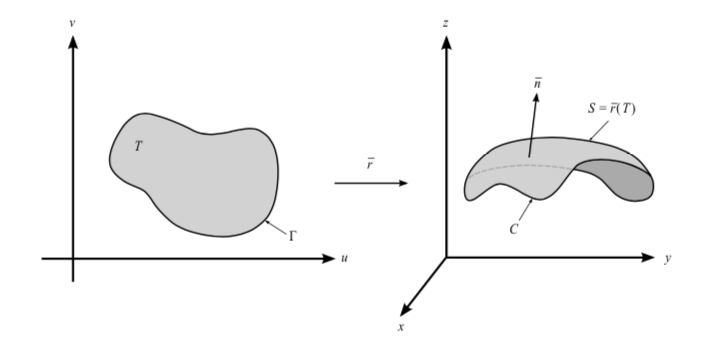
\includegraphics[scale=0.7]{Imagenes/Teoremas_Integrales_01.png}
    \caption{Aplicación del teorema de Stokes.}
    \label{fig:figura_01}
\end{figure}
\subsection{Teorema de Stokes.}
\begin{teo}Teorema de Stokes.

Sea $S = \overline{r}(T)$ una superficie paramétrica regular simple, donde $T$ es una región del plano $OUV$ limitada por una curva de Jordan $\Gamma$  descrita por un camino regular a trozos $\overline{\gamma}$. Supongamos
también que $\overline{r}$ es una aplicación inyectiva de clase $C^{2}$ en un entorno abierto de $T \cup \Gamma$ . Sea $C$ la imagen de $\Gamma$ por $\overline{r}$, y sea $\overline{F} = (P, Q, R)$ un campo vectorial de clase $C^{1} (S)$. Entonces:
\begin{align*}
\iint_{S} (\curl{\overline{F}}) \cdot \dd{S} = \int_{C} \overline{F} \cdot \dd{\overline{\alpha}}
\end{align*}
donde $\overline{\alpha} = \overline{r} \circ \overline{\gamma}$ es una parametrización de $C$ y $\Gamma$ se recorre en sentido positivo.
\end{teo}
\begin{proof}

Sea $\overline{\gamma}$ la parametrización de $\Gamma$ dada por
\begin{align*}
\overline{\gamma}(t) = (U(t), V(t)) , \hspace{0.5cm} t \in [a, b]
\end{align*}
Si $\overline{F} = (P, Q, R)$, entonces
\begin{align*}
\text{rot} \, \overline{F} = \curl{F} = \left( \pdv{R}{y} - \pdv{Q}{z}, \pdv{P}{z} - \pdv{R}{x}, \pdv{Q}{x} - \pdv{P}{y} \right)
\end{align*}
Por otra parte, si
\begin{align*}
\overline{r} (u, v) = (X (u, v), Y(u, v), Z(u, v)) \hspace{1cm} (u, v) \in T
\end{align*}
entonces
\begin{align*}
\pdv{\overline{r}}{u} \cp \pdv{\overline{r}}{v} = \left( \pdv{(Y, Z)}{(u, v)}, \pdv{(Z, X)}{(u, v)}, \pdv{(X, Y)}{(u, v)} \right)
\end{align*}
Necesitamos demostrar que:
\begin{align*}
\iint_{S} (\curl{\overline{F}}) \cdot dd{S} &= \iint_{T} \left( \pdv{R}{y} - \pdv{Q}{z}, \pdv{P}{z} - \pdv{R}{x}, \pdv{Q}{x} - \pdv{P}{y} \right) \cdot \\[0.5em]
&\cdot \left( \pdv{(Y, Z)}{(u, v)}, \pdv{(Z, X)}{(u, v)}, \pdv{(X, Y)}{(u, v)} \right) \dd{u} \dd{v} \\
&= \int_{C} P \dd{x} + Q \dd{y} + R \dd{z}
\end{align*}
para esto, basta con demostras las siguientes tres igualdades:
\begin{align}
\begin{aligned}
\iint_{T} \left[ \pdv{P}{z} \, \pdv{(Z, X)}{(u, v)} - \pdv{P}{y} \, \pdv{(X, Y)}{(u, v)} \right] \dd{u} \dd{v} &= \int_{C} P \dd{x} \\[0.5em]
\iint_{T} \left[ \pdv{Q}{x} \, \pdv{(X, Y)}{(u, v)} - \pdv{Q}{z} \, \pdv{(Y, Z)}{(u, v)} \right] \dd{u} \dd{v} &= \int_{C} Q \dd{y} \\[0.5em]
\iint_{T} \left[ \pdv{R}{y} \, \pdv{(Y, Z)}{(u, v)} - \pdv{R}{x} \, \pdv{(Z, X)}{(u, v)} \right] \dd{u} \dd{v} &= \int_{C} R \dd{z}
\end{aligned}
\label{eq:ecuacion_01}
\end{align}
Nos ocuparemos solamente de establecer la primera de ellas, ya que las dos restantes admiten un tratamiento análogo.

\end{proof}
\end{document}